% !TeX program = xelatex
% Сборка из папки лабораторной: xelatex report_template.tex (два раза).
% Для собственного отчёта сохранить копию под именем report.tex.
\documentclass[12pt,a4paper]{article}
\usepackage{fontspec}
\usepackage{polyglossia}
\setdefaultlanguage{russian}
\setmainfont{Times New Roman}
\setmonofont{Courier New}
\newfontfamily\cyrillicfonttt[Script=Default]{Courier New}
\usepackage{amsmath,amssymb,graphicx,array}
\usepackage[margin=2cm]{geometry}
\usepackage{xcolor,listings}
\usepackage[unicode,hidelinks]{hyperref}
\setlength{\parindent}{0pt}
\setlength{\parskip}{6pt}
\setlength{\emergencystretch}{3em}
\renewcommand{\arraystretch}{1.25}
\newcommand{\taskhead}[1]{\par\textbf{#1}\par}
% Сохранять ASCII-дефис U+002D при копировании кода из PDF.
\lstset{literate={-}{{\char45}}1}
\lstdefinestyle{commands}{
  basicstyle=\ttfamily\small,
  backgroundcolor=\color{gray!10},
  frame=single,framerule=0pt,framesep=6pt,
  xleftmargin=6pt,xrightmargin=6pt,
  breaklines=true,columns=fullflexible,keepspaces=true,
  showstringspaces=false
}

\begin{document}
\begin{titlepage}
{\color{black!50}
\textbf{\textit{Примечание:}} В данном документе представлен сокращённый
образец оформления титульного листа и результатов выполнения лабораторной
работы только для некоторых задач (задача 1.1 и задачи раздела 2).
Приведены примеры оформления аналитических вычислений, вызова функции,
таблиц сравнения и тестирования, рисунков и выводов.
Сведения об участниках и номере варианта приведены для примера;
в расчётах использованы демонстрационные данные из условия.
\par}

\vspace{2cm}
{\large\bfseries Отчёт по лабораторной работе\par}

\textbf{По дисциплине:} Линейная алгебра и геометрия (1 семестр)

\textbf{На тему:} Системы линейных уравнений, кривые второго порядка
и векторное представление текстов

\vspace{2cm}

\textbf{Вариант № 1}

\textbf{Выполнили} студенты гр. № 123456:

\textit{Иванов И.И., Петров П.П., Сидоров С.С.}

\textbf{Дата выполнения:} [дата]

\vspace{1cm}
\textbf{Цель работы}

Изучение свойств определителя при элементарных преобразованиях строк
и роли замены координат в приведении уравнения кривой второго порядка
к каноническому виду.

\vspace{0.8cm}
\textbf{Условия выполнения}

ОС: macOS. Python 3.12.3. NumPy 2.2.6. Сборка отчёта: XeLaTeX.
Программные результаты проверены на демонстрационной реализации.
В собственном отчёте указываются фактическое окружение и результаты
проверки собственной реализации.
\end{titlepage}

\taskhead{Порядок выполнения}
\begin{enumerate}
\item[1.1] Определитель вычислен с помощью элементарных преобразований строк.
Полученный результат сопоставлен с результатом функции и проверен тестами.
\item[2.1] В уравнении кривой выполнены поворот осей и перенос начала координат.
Найдены характеристики эллипса и проверены две контрольные точки.
Построены графики в исходных и канонических координатах.
Результаты оформлены в таблицах и на рисунках.
\end{enumerate}

\newpage

\begingroup
\setlength{\parskip}{4pt}
\setlength{\abovedisplayskip}{6pt}
\setlength{\belowdisplayskip}{6pt}
\setlength{\textfloatsep}{8pt}
\setlength{\intextsep}{8pt}
\section{Определители, СЛАУ и координаты вектора}
\subsection{Вычисление определителя}
\taskhead{Исходные данные и аналитическое решение}
Использована матрица из разобранного примера условия:
\[
A=\begin{pmatrix}0&2&1\\1&1&0\\2&0&1\end{pmatrix}.
\]
Переставим первую и третью строки, затем вычтем из второй строки
половину первой:
\[
A\xrightarrow{R_1\leftrightarrow R_3}
\begin{pmatrix}2&0&1\\1&1&0\\0&2&1\end{pmatrix}
\xrightarrow{R_2\gets R_2-\frac12R_1}
\begin{pmatrix}2&0&1\\0&1&-\frac12\\0&2&1\end{pmatrix}.
\]
Для выбора ведущего элемента второго столбца переставим вторую
и третью строки. Обнулим оставшийся элемент под диагональю:
\[
\begin{pmatrix}2&0&1\\0&1&-\frac12\\0&2&1\end{pmatrix}
\xrightarrow{R_2\leftrightarrow R_3}
\begin{pmatrix}2&0&1\\0&2&1\\0&1&-\frac12\end{pmatrix}
\xrightarrow{R_3\gets R_3-\frac12R_2}
U=\begin{pmatrix}2&0&1\\0&2&1\\0&0&-1\end{pmatrix}.
\]
Выполнены две перестановки. Строки не умножались на отдельные
множители; прибавления кратных строк определитель не изменили.
Поэтому
\[
z=\det A=(-1)^2\cdot2\cdot2\cdot(-1)=-4.
\]

\taskhead{Программный результат и сравнение}
После реализации функции в \texttt{solution.py} её вызов
из \texttt{variant\_check.py} имеет вид:
\begin{lstlisting}[style=commands]
from solution import determinant

matrix = [[0, 2, 1], [1, 1, 0], [2, 0, 1]]
print(determinant(matrix))  # -4.0
\end{lstlisting}
Для проверенной реализации $\widehat z=-4.0$. Ошибки вычислены
до округления:
\[
\Delta=|\widehat z-z|=|-4-(-4)|=0,\qquad
\delta=\frac{\Delta}{|z|}=\frac{0}{4}=0.
\]
Результаты сопоставлены в таблице~\ref{tab:errors}.
\begin{table}[htbp]
\centering
\caption{Сравнение аналитического и программного определителей}
\label{tab:errors}
\begin{tabular}{|l|r|r|r|r|}\hline
Величина & Аналитически & Программа & Абс. ошибка & Отн. ошибка\\\hline
$\det A$ & $-4$ & $-4.000000$ & $0$ & $0$\\\hline
\end{tabular}
\end{table}

Итоги тестирования приведены в таблице~\ref{tab:tests}.

\taskhead{Вывод} 

Аналитический и программный результаты совпали.
Абсолютная ошибка меньше $10^{-8}$. В задаче вычисления определителя
невязка системы уравнений не определяется.

\clearpage
\endgroup
\section{Приведение кривой второго порядка к каноническому виду}
\taskhead{Исходное уравнение и поворот координатных осей}
Рассмотрено уравнение из разобранного примера условия:
\[
F(x,y)=5x^2-6xy+5y^2-14x+2y-3=0.
\]
Смешанный член $-6xy$ устраняется поворотом осей.
При $x=r\cos\theta$, $y=r\sin\theta$ квадратичная часть равна
$r^2(5-3\sin2\theta)$.
Выберем $\theta=\psi+\pi/4$ и положим
$s=r\cos\psi$, $t=r\sin\psi$. Тогда
\[
r^2(5-3\cos2\psi)=2s^2+8t^2,\qquad
x=\frac{s-t}{\sqrt2},\quad y=\frac{s+t}{\sqrt2}.
\]
Линейные члены преобразуются по тем же формулам:
\[
-14x+2y=\frac{-14(s-t)+2(s+t)}{\sqrt2}
=-6\sqrt2s+8\sqrt2t.
\]
Получено уравнение без смешанного члена:
\[
2s^2+8t^2-6\sqrt2s+8\sqrt2t-3=0.
\]

\taskhead{Выделение квадратов и перенос начала координат}
\begin{align*}
2s^2-6\sqrt2s&=2\left(s-\frac{3\sqrt2}{2}\right)^2-9,\\
8t^2+8\sqrt2t&=8\left(t+\frac{\sqrt2}{2}\right)^2-4.
\end{align*}
После подстановки и переноса постоянных слагаемых:
\[
2\left(s-\frac{3\sqrt2}{2}\right)^2+
8\left(t+\frac{\sqrt2}{2}\right)^2=16.
\]
Введём $u=s-3\sqrt2/2$, $v=t+\sqrt2/2$. Каноническое уравнение:
\[
\boxed{\frac{u^2}{8}+\frac{v^2}{2}=1}.
\]
Прямой и обратный переходы между координатами имеют вид
\[
\begin{cases}u=(x+y-3)/\sqrt2,\\v=(-x+y+1)/\sqrt2,\end{cases}
\qquad
\begin{cases}x=2+(u-v)/\sqrt2,\\y=1+(u+v)/\sqrt2.\end{cases}
\]
Кривая является эллипсом с центром $C=(2,1)$ и полуосями
$a=2\sqrt2$, $b=\sqrt2$. Направления большой и малой осей
в исходных координатах заданы векторами $(1,1)$ и $(-1,1)$.

\taskhead{Проверка контрольных точек}
Для точки $A$: $(u,v)=(2\sqrt2,0)$ имеем $8/8=1$,
а исходные координаты равны $(4,3)$. Подстановка даёт
\[
F(4,3)=80-72+45-56+6-3=0.
\]
Для точки $B$: $(u,v)=(0,\sqrt2)$ имеем $2/2=1$,
а исходные координаты равны $(1,2)$. Подстановка даёт
\[
F(1,2)=5-12+20-14+4-3=0.
\]

\clearpage
\taskhead{Графическая проверка}
На рисунке~\ref{fig:original} представлен эллипс в исходных
координатах, на рисунке~\ref{fig:canonical} --- в канонических.
На обоих рисунках отмечены центр $C$, контрольные точки $A$, $B$
и остальные вершины эллипса. Пунктирные стрелки на первом рисунке
показывают положительные направления новых осей.
Масштаб по горизонтальной и вертикальной осям одинаков.

% Для собственных графиков заменить пути, сохранив относительные имена.
% Каждый рисунок имеет подпись и метку для ссылки через \ref.
\begin{figure}[htbp]
\centering
\begin{minipage}[t]{0.49\textwidth}
\centering
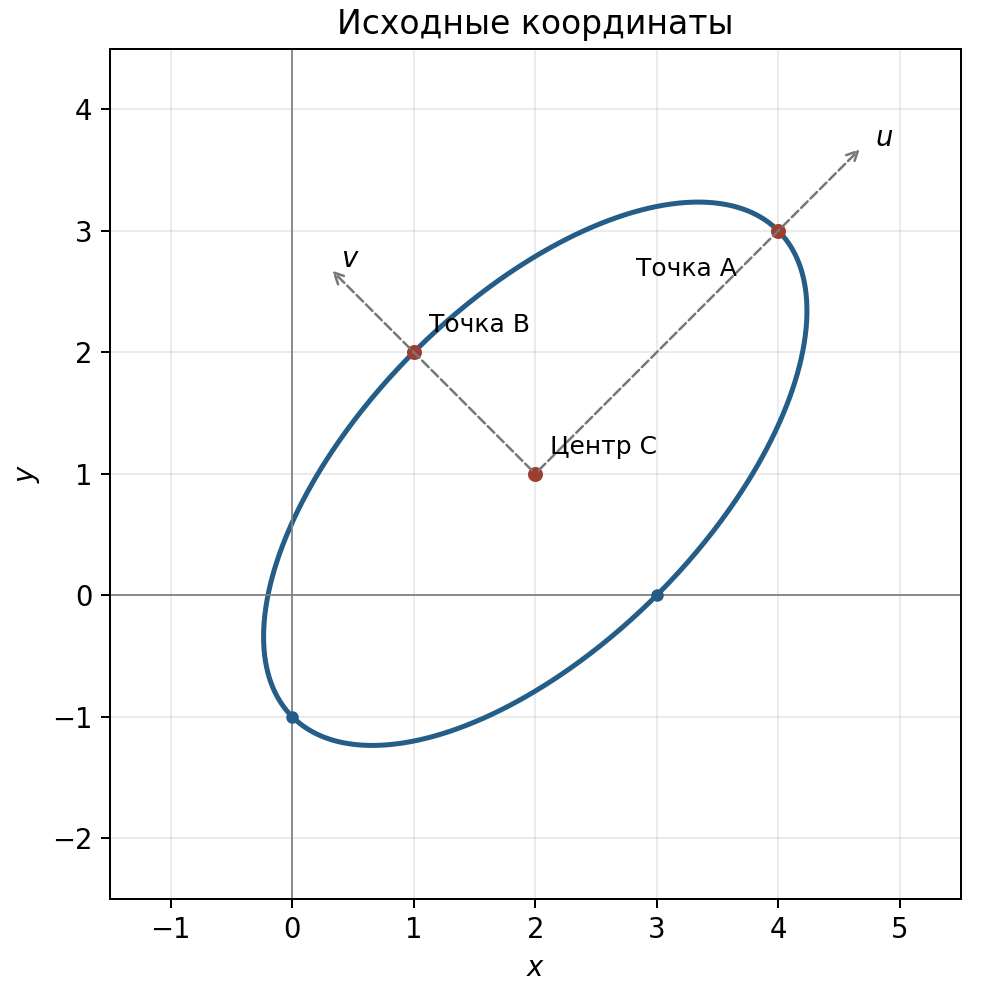
\includegraphics[width=\linewidth]{examples/report_figures/original_curve.png}
\caption{Эллипс в исходной системе координат $(x,y)$}
\label{fig:original}
\end{minipage}\hfill
\begin{minipage}[t]{0.49\textwidth}
\centering
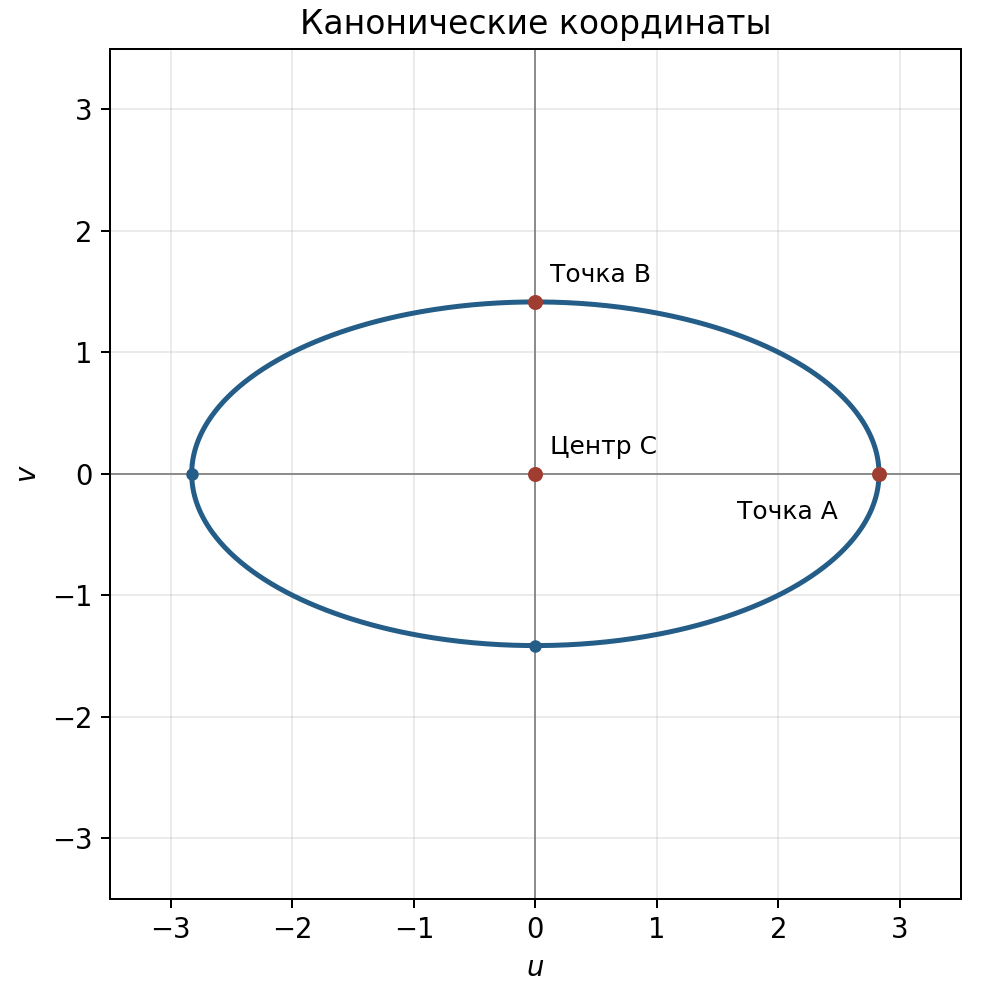
\includegraphics[width=\linewidth]{examples/report_figures/canonical_curve.png}
\caption{Эллипс в канонической системе координат $(u,v)$}
\label{fig:canonical}
\end{minipage}
\end{figure}

\taskhead{Вывод} 

Графики согласуются с аналитическим решением:
центр исходной кривой расположен в точке $(2,1)$,
после замены координат --- в начале координат.
Большая полуось направлена вдоль оси $u$, малая --- вдоль оси $v$.
Проверки обеих контрольных точек дали нулевые значения исходного полинома.
Программное приведение к каноническому виду не выполнялось.

\taskhead{Проверка реализации}
Таблица~\ref{tab:tests} содержит итог проверки демонстрационной
реализации на четырёх тестах группы \texttt{determinant}.
\begin{table}[htbp]
\centering
\caption{Результаты тестирования}
\label{tab:tests}
\small
\begin{tabular}{|l|p{8.2cm}|l|c|}\hline
Задача & Команда запуска & Статус & Пройдено\\\hline
Определитель & \texttt{python run.py unittest determinant} & Успешно & 4 из 4\\\hline
\end{tabular}
\end{table}

\clearpage
\section*{Заключение по лабораторной работе}
В задаче 1.1 получен определитель $-4$, подтверждённый программным
вычислением и тестированием. В разделе 2 аналитически получено
каноническое уравнение эллипса; замены координат проверены подстановкой
и графически. Расхождений в выполненных проверках не обнаружено.

\section*{Источник исходных данных}
Условие лабораторной работы, файл \texttt{main.tex}: примеры
в задаче 1.1 и разделе 2. В полном отчёте дополнительно указываются
фактически использованные внешние источники.
\end{document}
